\documentclass[11pt]{article}
\usepackage{fontspec}\setmonofont{DejaVu Sans Mono}[Scale=0.8]
\usepackage{amsmath,amssymb}\usepackage[margin=1in]{geometry}
\usepackage{fancyvrb}\usepackage[hidelinks]{hyperref}\usepackage{enumitem}
\usepackage{graphicx}\usepackage{float}
\usepackage{newunicodechar}
\newunicodechar{μ}{\ensuremath{\mu}}
\newunicodechar{∂}{\ensuremath{\partial}}
\newunicodechar{Τ}{\ensuremath{\mathrm{T}}}
\newunicodechar{ρ}{\ensuremath{\rho}}
\newunicodechar{Ψ}{\ensuremath{\Psi}}
\setlist{nosep,leftmargin=1.4em}
\newcommand{\Tau}{\mathrm{T}}
\IfFontExistsTF{Noto Sans Egyptian Hieroglyphs}{\newfontfamily{\egyptian}{Noto Sans Egyptian Hieroglyphs}}{\newcommand{\egyptian}{}}
\IfFontExistsTF{Noto Sans Cuneiform}{\newfontfamily{\cuneiform}{Noto Sans Cuneiform}}{\newcommand{\cuneiform}{}}
\newcommand{\glyph}[1]{\text{\egyptian #1}}
\newcommand{\cunei}[1]{\text{\cuneiform #1}}
\title{Proposing Models, Inference, and Provenance: State Summary and Enacting}\author{Brent Hartshorn\\ \texttt{brenthartshorn@proton.me}}
\date{Stage 12 \quad (parent: doi:local:self\_11)}
\begin{document}\maketitle
\begin{abstract}Stage 12 of a self-evolving hypergraph, extended from its parent (doi:local:self\_11) so the inquiry can look fully back. It declares 9 nodes, each pairing a suggestive Greek glyph with a precise description. Of these, 2 compile via @dslai into small trainable modules (Sigma, Psi), making the hypergraph partly differentiable; a module computes, it does not comprehend. It also reads its own published lineage --- opening 12 ancestor stages and tracing where each term entered --- and records that provenance as data, not as self-understanding. A circuit equation compiles 6 trainable networks --- one bound to each symbol --- and wires them into 2 composite(s); the equation builds the networks, and the numbers they return are data, not the symbols' meanings combining. It posits 5 fuzzy axioms and 3 large laws over the terms, with memberships taken from the relation geometry; each law evaluates to a number in [0,1] recorded as data --- the degree to which an authored postulate holds, not a truth about a self. It inscribes the formal measurements of the companion paper on matrix inscriptions: co-occurrence geometry and Laplacian spectrum, circuit Jacobians as matrix products, and provenance as a filtration with birth times --- each a deterministic function of authored data. An oracle increment may extend the hypergraph programmatically; the engine records what was proposed as data beside the questions, not as answers. It may search outward (arXiv), fetch allowlisted PDFs into a local corpus, ingest excerpts, and propose module architectures --- each operation returns bibliographic or textual data and authored proposals, not comprehension of a self. It relates them by 15 binary relations and 13 hyperedges, and may trigger gated actions whose output is recorded as data, never as an answer. The engine, introspected from its own source, exposes act\_coherence, act\_neural, compile\_module, forward, train, act\_train, act\_infer, read\_lineage, lineage\_search, act\_provenance, act\_circuit, act\_geometry, act\_jacobian, act\_filtration, act\_spectrum, act\_oracle, act\_search, act\_fetch, act\_ingest, act\_propose, act\_law, parse, to\_questions, title, abstract, run\_actions, build\_tex, build\_pdf, state\_summary, build\_prompt, apply\_oracle, evolve\_auto, evolve. It poses questions and enacts computations beside them; it makes no claim to resolve what a self is.\end{abstract}
\section*{Symbolic core (inherited relations)}\begin{align*}
\Omega \; \longrightarrow \; \Sigma \\[3pt] \Sigma \; \models \; \Sigma \\[3pt] \Sigma \; \otimes \; \Lambda \\[3pt] \partial \Sigma \; \stackrel{?}{=} \; \mu \\[3pt] \Sigma \; \nprec \; \Omega \\[3pt] \Phi \; \longrightarrow \; \Sigma \\[3pt] \Phi \; \rightsquigarrow \; \Sigma \\[3pt] \Tau \; \Rrightarrow \; \Lambda \\[3pt] \partial \Lambda \; \rightsquigarrow \; \mu \\[3pt] \Delta \; \dashrightarrow \; \mu \\[3pt] \partial \Tau \; \otimes \; \Delta \\[3pt] \Psi \; \leadsto \; \Sigma \\[3pt] \rho \; \otimes \; \Lambda \\[3pt] \Psi \; \leadsto \; \rho \\[3pt] \partial \rho \; \stackrel{?}{=} \; \Omega
\end{align*}
\section*{Circuit (a new equation that wires several networks)}Beyond the inherited relations, this stage adds an equation that binds a small trainable network to \emph{each} symbol and composes them along the arrow:\begin{equation*}\Sigma \;=\; \Phi \longrightarrow \Lambda \longrightarrow \mu \qquad (\text{width } 5)\\[4pt] \rho \;=\; \Psi \longrightarrow \Lambda \longrightarrow \mu \qquad (\text{width } 4)\end{equation*}Each such equation compiles to 6 trainable networks (one per symbol), wired into a composite. Building the networks is what the equation does; the training losses and outputs the composite returns are recorded as data, not the symbols' meanings combining.
\section*{Nodes (suggestive glyph + precise description)}
\begin{description}\item[$ \Omega $] origin --- \emph{that from which the self is said to come}
\item[$ \Sigma $] self --- \emph{the locus that poses and is altered by the question} \quad $\rightarrow$ \texttt{module 2->2->2 (sigmoid), trainable}
\item[$ \Lambda $] language --- \emph{the finite medium any self must pass through}
\item[$ \mu $] meaning --- \emph{what a reader supplies, or finds, in the passage}
\item[$ \Phi $] other --- \emph{the one whose regard first gives the self to itself}
\item[$ \Tau $] time --- \emph{the direction in which the self cannot return}
\item[$ \Delta $] difference --- \emph{the gap that lets one thing be told from another}
\item[$ \Psi $] oracle --- \emph{the voice that proposes beside the question without claiming to answer} \quad $\rightarrow$ \texttt{module 3->4->3 (sigmoid), trainable}
\item[$ \rho $] field --- \emph{the outward literature the inquiry reads without claiming to understand}\end{description}
\section*{Hypergraph (questions, and the data actions returned)}
\begin{itemize}\item $\{\Sigma\}$ \quad \textbf{?} Can the self reconstruct itself from its own compression? \quad[\texttt{train}]\\ \hspace*{1em}$\hookrightarrow$ \emph{recorded data (not an answer):} \texttt{\{'node': 'Sigma', 'arch': '2->2->2', 'task': 'autoencode', 'mse\_start': 0.0549, 'mse\_final': 0.011, 'weights\_from\_symbols': True, 'params': 12, 'symbolic\_roundtrip\_err': 0.000196, 'is': 'an optimization result over a defined toy objective, with the trained weights written to the appendix as glyphs; not the self learning what it is'\}}
\item $\{\Omega,\,\Sigma,\,\Lambda\}$ \quad \textbf{?} Where, in this inquiry's own history, did origin, self, and language first enter? \quad[\texttt{provenance}]\\ \hspace*{1em}$\hookrightarrow$ \emph{recorded data (not an answer):} \texttt{\{'provenance': \{'Omega': \{'word': 'origin', 'entered': 'stage 0', 'seen\_in': ['0', '1', '10', '11', '2', '3', '4', '5', '6', '7', '8', '9'], 'n\_relations': 24\}, 'Sigma': \{'word': 'self', 'entered': 'stage 0', 'seen\_in': ['0', '1', '10', '11', '2', '3', '4', '5', '6', '7', '8', '9'], 'n\_relations': 83\}, 'Lambda': \{'word': 'language', 'entered': 'stage 0', 'seen\_in': ['0', '1', '10', '11', '2', '3', '4', '5', '6', '7', '8', '9'], 'n\_relations': 32\}\}, 'is': 'a citation of the lineage; where terms entered, not what they mean'\}}
\item $\{\Phi,\,\Lambda,\,\mu,\,\Sigma\}$ \quad \textbf{?} If a self is wired from other, language, and meaning, what does the composite return? \quad[\texttt{circuit}]\\ \hspace*{1em}$\hookrightarrow$ \emph{recorded data (not an answer):} \texttt{\{'circuit': \{'Sigma': \{'wiring': 'Phi -> Lambda -> mu', 'networks': \{'Phi': \{'arch': '5->5->5', 'trained\_mse': 0.0683\}, 'Lambda': \{'arch': '5->5->5', 'trained\_mse': 0.057\}, 'mu': \{'arch': '5->5->5', 'trained\_mse': 0.0586\}\}, 'n\_networks': 3, 'composite\_output\_norm': 1.192\}, 'rho': \{'wiring': 'Psi -> Lambda -> mu', 'networks': \{'Psi': \{'arch': '4->4->4', 'trained\_mse': 0.07\}, 'Lambda': \{'arch': '4->4->4', 'trained\_mse': 0.0672\}, 'mu': \{'arch': '4->4->4', 'trained\_mse': 0.0685\}\}, 'n\_networks': 3, 'composite\_output\_norm': 1.077\}\}, 'is': "several trained networks wired by the equation; the numbers are data, not the symbols' meanings combining"\}}
\item $\{\Sigma,\,\Phi,\,\Lambda,\,\mu,\,\Delta,\,\Tau\}$ \quad \textbf{?} To what degree do the authored laws of the self hold under the geometry? \quad[\texttt{law}]\\ \hspace*{1em}$\hookrightarrow$ \emph{recorded data (not an answer):} \texttt{\{'law': \{'constitution': 0.47, 'dissolution': 0.61, 'self': 0.09\}, 'memberships': \{'Omega': 0.41, 'Sigma': 1.0, 'Lambda': 0.59, 'mu': 0.54, 'Phi': 0.47, 'Tau': 0.39, 'Delta': 0.38, 'Psi': 0.12, 'rho': 0.07\}, 'is': 'the degree to which each authored law holds under degree-derived memberships; numbers in [0,1], not truths about a self'\}}
\item $\{\Omega,\,\Sigma,\,\Lambda,\,\mu,\,\Phi,\,\Tau,\,\Delta\}$ \quad \textbf{?} What is the geometry of the relations — and which term is the hub? \quad[\texttt{geometry}]\\ \hspace*{1em}$\hookrightarrow$ \emph{recorded data (not an answer):} \texttt{\{'degrees': \{'Omega': 45, 'Sigma': 109, 'Lambda': 64, 'mu': 59, 'Phi': 51, 'Tau': 42, 'Delta': 41, 'Psi': 13, 'rho': 8\}, 'hub': 'Sigma', 'laplacian\_smallest\_nonzero': 8.615421, 'laplacian\_fiedler': 8.615421, 'is': 'a map of the authored relation structure; hub centrality is a fact about what was written, not a fact about selves'\}}
\item $\{\Phi,\,\Lambda,\,\mu,\,\Sigma\}$ \quad \textbf{?} If the circuit is composed, what is the Jacobian of the composite at a point? \quad[\texttt{jacobian}]\\ \hspace*{1em}$\hookrightarrow$ \emph{recorded data (not an answer):} \texttt{\{'jacobian': \{'Sigma': \{'wiring': 'Phi -> Lambda -> mu', 'jacobian\_norm': 0.0001, 'jacobian\_shape': [5, 5], 'is': 'the matrix product of per-module Jacobians; composition of maps, not combination of meanings'\}, 'rho': \{'wiring': 'Psi -> Lambda -> mu', 'jacobian\_norm': 0.0, 'jacobian\_shape': [4, 4], 'is': 'the matrix product of per-module Jacobians; composition of maps, not combination of meanings'\}\}, 'is': 'chain-rule Jacobians of the circuit composite; data, not semantics'\}}
\item $\{\Omega,\,\Phi,\,\Tau,\,\Delta\}$ \quad \textbf{?} At which stage did each term enter the lineage? \quad[\texttt{filtration}]\\ \hspace*{1em}$\hookrightarrow$ \emph{recorded data (not an answer):} \texttt{\{'filtration': \{'Omega': \{'word': 'origin', 'birth\_time': 0, 'iota': 'stage 0'\}, 'Phi': \{'word': 'other', 'birth\_time': 1, 'iota': 'stage 1'\}, 'Tau': \{'word': 'time', 'birth\_time': 10, 'iota': 'stage 10'\}, 'Delta': \{'word': 'difference', 'birth\_time': 10, 'iota': 'stage 10'\}\}, 'is': 'birth times along the monotone chain; citations with dates, not meanings'\}}
\item $\{\Omega,\,\Sigma,\,\Lambda,\,\mu,\,\Phi,\,\Tau,\,\Delta,\,\Psi\}$ \quad \textbf{?} Where does each term sit in the spectral embedding of the relation Laplacian? \quad[\texttt{spectrum}]\\ \hspace*{1em}$\hookrightarrow$ \emph{recorded data (not an answer):} \texttt{\{'spectrum': \{'Omega': [-0.124, -0.0898], 'Sigma': [-0.1159, -0.0636], 'Lambda': [-0.1211, -0.1112], 'mu': [-0.1367, -0.1113], 'Phi': [-0.1501, -0.0918], 'Tau': [-0.1756, -0.1324], 'Delta': [-0.1802, -0.133], 'Psi': [0.0846, 0.937]\}, 'fiedler\_value': 8.615421, 'is': 'a spectral embedding of the co-occurrence matrix; coordinates are functions of M, not discoveries about selves'\}}
\item $\{\Psi,\,\Sigma\}$ \quad \textbf{?} What increment did the oracle propose for this stage — and what changed? \quad[\texttt{oracle}]\\ \hspace*{1em}$\hookrightarrow$ \emph{recorded data (not an answer):} \texttt{\{'oracle': \{'new\_terms': ['rho'], 'new\_relations': ['rho (x) Lambda', 'Psi <\textasciitilde{} rho', '@rho ?= Omega'], 'new\_hyperedges': 4, 'new\_actions': ['fetch', 'ingest', 'propose', 'search'], 'stage': '12', 'summary': '+1 term(s), +3 relation(s), +4 hyperedge(s)'\}, 'is': 'a record of the authored increment; the proposal stands beside the question, not in place of an answer'\}}
\item $\{\rho,\,\Lambda,\,\Sigma\}$ \quad \textbf{?} What outward papers speak to origin, language, and self? \quad[\texttt{search}]\\ \hspace*{1em}$\hookrightarrow$ \emph{recorded data (not an answer):} \texttt{\{'search': \{'queries': ['self field language self the the neuro-symbolic', 'neuro-symbolic self-modifying DSL', 'introspective knowledge generation emergent DSL', 'self-evolving hypergraph provenance', 'machine language emergence neural symbolic'], 'n\_hits': 12, 'hits': [\{'id': '1411.6643v4', 'title': 'Quantum memories at finite temperature', 'summary': 'To use quantum systems for technological applications we first need to preserve their coherence for macroscopic timescales, even at finite temperature. Quantum error correction has made it possible to actively correct errors that affect a quantum memory. An attractive scenario is the construction of passive storage of quantum information with minimal active support. Indeed, passive protection is t', 'pdf\_url': 'https://arxiv.org/pdf/1411.6643v4.pdf', 'is': 'a bibliographic hit from arXiv; not evidence about a self'\}, \{'id': '2509.02918v1', 'title': 'Single Domain Generalization in Diabetic Retinopathy: A Neuro-Symbolic Learning Approach', 'summary': 'Domain generalization remains a critical challenge in medical imaging, where models trained on single sources often fail under real-world distribution shifts. We propose KG-DG, a neuro-symbolic framework for diabetic retinopathy (DR) classification that integrates vision transformers with expert-guided symbolic reasoning to enable robust generalization across unseen domains. Our approach leverages', 'pdf\_url': 'https://arxiv.org/pdf/2509.02918v1.pdf', 'is': 'a bibliographic hit from arXiv; not evidence about a self'\}, \{'id': '1307.7872v1', 'title': 'Generating functionals for guided self-organization', 'summary': "Time evolution equations for dynamical systems can often be derived from generating functionals. Examples are Newton's equations of motion in classical dynamics which can be generated within the Lagrange or the Hamiltonian formalism. We propose that generating functionals for self-organizing complex systems offer several advantages. Generating functionals allow to formulate complex dynamical syste", 'pdf\_url': 'https://arxiv.org/pdf/1307.7872v1.pdf', 'is': 'a bibliographic hit from arXiv; not evidence about a self'\}, \{'id': '2412.15588v1', 'title': 'NeSyCoCo: A Neuro-Symbolic Concept Composer for Compositional Generalization', 'summary': 'Compositional generalization is crucial for artificial intelligence agents to solve complex vision-language reasoning tasks. Neuro-symbolic approaches have demonstrated promise in capturing compositional structures, but they face critical challenges: (a) reliance on predefined predicates for symbolic representations that limit adaptability, (b) difficulty in extracting predicates from raw data, an', 'pdf\_url': 'https://arxiv.org/pdf/2412.15588v1.pdf', 'is': 'a bibliographic hit from arXiv; not evidence about a self'\}, \{'id': '2506.01121v1', 'title': 'Neuro-Symbolic Generative Diffusion Models for Physically Grounded, Robust, and Safe Generation', 'summary': 'Despite the remarkable generative capabilities of diffusion models, their integration into safety-critical or scientifically rigorous applications remains hindered by the need to ensure compliance with stringent physical, structural, and operational constraints. To address this challenge, this paper introduces Neuro-Symbolic Diffusion (NSD), a novel framework that interleaves diffusion steps with ', 'pdf\_url': 'https://arxiv.org/pdf/2506.01121v1.pdf', 'is': 'a bibliographic hit from arXiv; not evidence about a self'\}, \{'id': '1109.0778v1', 'title': 'Building-Blocks for Performance Oriented DSLs', 'summary': 'Domain-specific languages raise the level of abstraction in software development. While it is evident that programmers can more easily reason about very high-level programs, the same holds for compilers only if the compiler has an accurate model of the application domain and the underlying target platform. Since mapping high-level, general-purpose languages to modern, heterogeneous hardware is bec', 'pdf\_url': 'https://arxiv.org/pdf/1109.0778v1.pdf', 'is': 'a bibliographic hit from arXiv; not evidence about a self'\}]\}, 'is': 'outward search results; titles and ids, not understanding'\}}
\item $\{\rho\}$ \quad \textbf{?} Which allowlisted PDFs were retrieved and stored beside the inquiry? \quad[\texttt{fetch}]\\ \hspace*{1em}$\hookrightarrow$ \emph{recorded data (not an answer):} \texttt{\{'downloaded': [\{'source': 'vixra', 'id': '2507.0104', 'title': 'Towards Self-Evolving AGI via Emergent DSL', 'path': 'corpus/2507.0104v1.pdf'\}, \{'source': 'vixra', 'id': '2507.0074', 'title': 'Self-Contained Multi-AI Architecture Definition via DSL', 'path': 'corpus/2507.0074v1.pdf'\}, \{'source': 'vixra', 'id': '2507.0036', 'title': 'Emergent Self-Modification and Meta-Programming', 'path': 'corpus/2507.0036v1.pdf'\}, \{'source': 'arxiv', 'id': '1411.6643v4', 'title': 'Quantum memories at finite temperature', 'path': 'corpus/1411.6643v4.pdf'\}, \{'source': 'arxiv', 'id': '2509.02918v1', 'title': 'Single Domain Generalization in Diabetic Retinopathy: A Neuro-Symbolic Learning Approach', 'path': 'corpus/2509.02918v1.pdf'\}, \{'source': 'arxiv', 'id': '1307.7872v1', 'title': 'Generating functionals for guided self-organization', 'path': 'corpus/1307.7872v1.pdf'\}], 'errors': [], 'corpus\_dir': 'corpus', 'is': 'files stored beside the inquiry; storage, not comprehension'\}}
\item $\{\rho,\,\mu\}$ \quad \textbf{?} What phrases survive when the corpus is carried toward meaning? \quad[\texttt{ingest}]\\ \hspace*{1em}$\hookrightarrow$ \emph{recorded data (not an answer):} \texttt{\{'snippets': [\{'file': '1307.7872v1.pdf', 'term\_hits': 2, 'excerpt': 'iment. One may then expect, thanks to Darwinian selection, that the such co nstructed dynamical equation should exhibit meaningful behavior, replicating observations. • Exploring Phase Space A complete understanding would correspond, within dynamic al system theory, to a full control of both the qualitative behavior of the flow in p hase space and of its dependency on the control parameters. Achieving this kind o f complete control is clearly very desirable, but often extremely hard to achievewhen dealing with large numbers of dynamical variables and control parameters, the typical situation in modern complex system theory. The exploration of phase space, typically through a combination of analytical and numerical investigations, is in any case an indis- pensable tool, even when only a smal', 'is': 'extracted text; co-occurrence with authored terms, not meaning'\}, \{'file': '1411.6643v4.pdf', 'term\_hits': 0, 'excerpt': 'Quantum memories at finite temperature Benjamin J. Brown, 1, 2 Daniel Loss, 3 Jiannis K. Pachos, 4 Chris N. Self, 1, 4 and James R. Wootton 3 1Quantum Optics and Laser Science, Blackett Laboratory, Imperial College London, Prince Consort Road, London, SW7 2AZ, United Kingdom 2Niels Bohr International Academy, Niels Bohr Institute, Blegdamsvej 17, 2100 Copenhagen, Denmark 3Department of Physics, University of Basel, Klingelbergstrasse 82, CH-4056 Basel, Switzerland 4School of Physics and Astronomy, University of Leeds, Leeds LS2 9JT, United Kingdom To use quantum systems for technological applications we first need to preserve their coherence for macroscopic timescales, even at finite temperature. Quantum error correction has made it possible to actively correct errors that affect a quantum mem', 'is': 'extracted text; co-occurrence with authored terms, not meaning'\}, \{'file': '2507.0036v1.pdf', 'term\_hits': 2, 'excerpt': "ems Brent Hartshorn: July 7th, 2025 brenthartshorn@proton.me Abstract This paper presents a profound advancement in the field of emergent computation by demonstrating a novel system capable of dynamically  modifying its own core functionality. Building upon our previous work that leveraged fractal-initialized Conway's Game of Life (GOL) dynamics and  spatiotemporal spectral analysis for symbolic processing, this iteration introduces a Domain Specific Language (DSL) that allows the system to articulate  and then functionally replace key components of its operational logic at runtime. Specifically, we show how a neural network, through its spectral  interpretation of GOL dynamics, can generate DSL expressions that are compiled into executable Python code, effectively enabling the system to l", 'is': 'extracted text; co-occurrence with authored terms, not meaning'\}, \{'file': '2507.0074v1.pdf', 'term\_hits': 0, 'excerpt': "Self Contained Multi-AI Architecture Definition via DSL Brent Hartshorn July 13th Abstract This paper presents a significant evolution in emergent computational systems, extending the Domain-Specific Language (DSL) driven self- modification paradigm to encompass foundational components beyond neural network architectures and cellular automata rules. Building on prior work  where the AI could define its Game of Life (GOL) stepping function and classifier network via a tokenized DSL, we now demonstrate the system's  capacity to articulate and dynamically replace its fractal generation algorithms (e.g., Burning Ship and Mandelbrot). By expressing these complex  mathematical functions within the same learnable DSL, the system gains a deeper level of meta-programming, enabling the AI to not onl", 'is': 'extracted text; co-occurrence with authored terms, not meaning'\}, \{'file': '2507.0104v1.pdf', 'term\_hits': 4, 'excerpt': 'such as our GOL-based computational environment, generate high-dimensional data streams. To enable more efficient and  meaningful processing for the Classifier network, we have integrated Uniform Manifold Approximation and Projection (UMAP) for dynamic  dimensionality reduction. UMAP, a non-linear dimensionality reduction technique, is particularly adept at preserving both local and global data structures,  making it suitable for complex, high-dimensional inputs [6]. In our system, the previous history of output energy bands from the spectral GOL analysis, represented as high-dimensional vectors, is fed into  the UMAP algorithm. The output of UMAP , typically a 32-dimensional embedding (controlled by the --umap flag, setting NUM\_INPUT\_SPACE to 32), is then directly provided to the last 32 ', 'is': 'extracted text; co-occurrence with authored terms, not meaning'\}, \{'file': '2509.02918v1.pdf', 'term\_hits': 10, 'excerpt': 'o diverse backbones and datasets. 2.1 Domain Generalization In many real-world applications, particularly in biomedical fields, it is unrealistic to expect access to new patients’ data before model deployment due to domain shifts between data from different patients [38]. To address this challenge, the concept of Domain Generalization (DG) was introduced [5]. DG aims to train models on data from one or more related but distinct source domains, enabling them to generalize effectively to unseen, out-of-distribution (OOD) target domains. Since its formal introduction by Blanchard et al. in 2011 [5], a wide range of techniques have been proposed to tackle the DG challenge [71]–[6]. These approaches include learning domain-invariant representations by aligning source domain distributions [ 30, ', 'is': 'extracted text; co-occurrence with authored terms, not meaning'\}], 'files': ['1307.7872v1.pdf', '1411.6643v4.pdf', '2507.0036v1.pdf', '2507.0074v1.pdf', '2507.0104v1.pdf', '2509.02918v1.pdf'], 'n\_files': 6, 'is': 'corpus ingest; phrases beside the question, not an answer'\}}
\item $\{\Psi,\,\Sigma,\,\rho\}$ \quad \textbf{?} What module architecture does the oracle propose from field and hub geometry? \quad[\texttt{propose}]\\ \hspace*{1em}$\hookrightarrow$ \emph{recorded data (not an answer):} \texttt{\{'proposals': [\{'node': 'Sigma', 'arch': '2->4->2', 'activation': 'sigmoid', 'task': 'autoencode', 'note': 'wider hidden layer beside low law\_self score; proposal only'\}, \{'node': 'Psi', 'arch': '3->4->3', 'activation': 'sigmoid', 'task': 'autoencode', 'note': 'oracle module mirroring propose-side width; proposal only'\}, \{'circuit': 'rho = Psi -> Lambda -> mu', 'width': 4, 'note': 'field routed through language toward meaning; symbolic wiring only'\}], 'corpus\_keywords': ['dsl'], 'hub': 'Sigma', 'law\_self': 0.09, 'is': 'authored architecture suggestions over analysis + corpus; not evidence that a self or model was discovered'\}}\end{itemize}
\section*{Axioms and laws (fuzzy logic over the terms)}
Memberships are taken from the relation geometry, $\mu(\sigma)=d(\sigma)/\max_\tau d(\tau)$:\begin{equation*}\mu(\Sigma){=}1.00,\;\; \mu(\Lambda){=}0.59,\;\; \mu(\mu){=}0.54,\;\; \mu(\Phi){=}0.47,\;\; \mu(\Omega){=}0.41,\;\; \mu(\Tau){=}0.39,\;\; \mu(\Delta){=}0.38,\;\; \mu(\Psi){=}0.12,\;\; \mu(\rho){=}0.07\end{equation*}
\noindent\textbf{Axioms} (authored postulates, not verified truths):\begin{itemize}\item \textsc{genesis}: $\,\Omega \Rightarrow \Sigma\,$\item \textsc{alterity}: $\,\Sigma \Rightarrow \Phi\,$\item \textsc{mediation}: $\,\Sigma \Rightarrow \Lambda\,$\item \textsc{distinction}: $\,\Sigma \Rightarrow \Delta\,$\item \textsc{finitude}: $\,\Sigma \Rightarrow \Tau\,$\end{itemize}
\noindent\textbf{Laws.} Each large equation brings several terms together; the braces draw the reading. Each evaluates to a number in $[0,1]$ --- recorded as data, not as a verdict.
\begin{equation*}\Sigma \Longleftrightarrow \overbrace{\Omega \oplus \Phi}^{\text{given: by origin and by the other}} \otimes \underbrace{\Lambda \Rightarrow \mu}_{\text{reached: through language, toward meaning}}\end{equation*}
\begin{equation*}\neg \Sigma \Longleftarrow \overbrace{\Delta \otimes \mu}^{\text{difference shatters meaning}} \oplus \underbrace{\Tau \otimes \Lambda}_{\text{time writes upon language}}\end{equation*}
\begin{equation*}\Sigma = \underbrace{\Omega \oplus \Phi}_{\text{the given}} \otimes \overbrace{\Lambda \Rightarrow \mu}^{\text{the mediated}} \ominus \underbrace{\Delta \otimes \Tau}_{\text{the dissolving}}\end{equation*}
Under the memberships above, the laws evaluate to\begin{equation*}\textsc{constitution}\rightsquigarrow 0.470,\;\; \textsc{dissolution}\rightsquigarrow 0.610,\;\; \textsc{self}\rightsquigarrow 0.090\end{equation*}\noindent degrees to which authored postulates hold under authored memberships --- data, not truths about a self.
\section*{Questions this stage poses}\begin{itemize}\item Does Ω give rise to Σ — and what precedes Ω?
\item On what does Σ entailing Σ rest?
\item When Σ is carried by Λ, what survives and what is lost?
\item Is ∂Σ the same as μ, or is μ supplied by the reader?
\item If Σ does not reduce to Ω, where is the remainder?
\item Does Φ give rise to Σ — and what precedes Φ?
\item Does Φ haunt Σ — present as an absence?
\item What residue remains because Τ leaves a trace upon Λ?
\item Does ∂Λ haunt μ — present as an absence?
\item What collapses when Δ shatters the structure of μ?
\item When ∂Τ is carried by Δ, what survives and what is lost?
\item Does Ψ propose beside Σ without claiming to answer?
\item When ρ is carried by Λ, what survives and what is lost?
\item Does Ψ propose beside ρ without claiming to answer?
\item Is ∂ρ the same as Ω, or is Ω supplied by the reader?
\item Can the self reconstruct itself from its own compression?
\item Where, in this inquiry's own history, did origin, self, and language first enter?
\item If a self is wired from other, language, and meaning, what does the composite return?
\item To what degree do the authored laws of the self hold under the geometry?
\item What is the geometry of the relations — and which term is the hub?
\item If the circuit is composed, what is the Jacobian of the composite at a point?
\item At which stage did each term enter the lineage?
\item Where does each term sit in the spectral embedding of the relation Laplacian?
\item What increment did the oracle propose for this stage — and what changed?
\item What outward papers speak to origin, language, and self?
\item Which allowlisted PDFs were retrieved and stored beside the inquiry?
\item What phrases survive when the corpus is carried toward meaning?
\item What module architecture does the oracle propose from field and hub geometry?\end{itemize}
\section*{Lineage read (this stage searched its ancestors)}This stage read 12 ancestor stages (\,0, 1, 10, 11, 2, 3, 4, 5, 6, 7, 8, 9\,) from their embedded sources, tracing 8 terms and 121 relations across the lineage. For example: $ \Omega $ (origin, from stage 0), $ \Sigma $ (self, from stage 0), $ \Lambda $ (language, from stage 0), $ \mu $ (meaning, from stage 0), $ \Phi $ (other, from stage 1). This is provenance retrieval --- where terms entered and what was said --- recorded as data, not a claim to understand the lineage.
\section*{Manifold (the geometry of the relations)}
\begin{figure}[H]\centering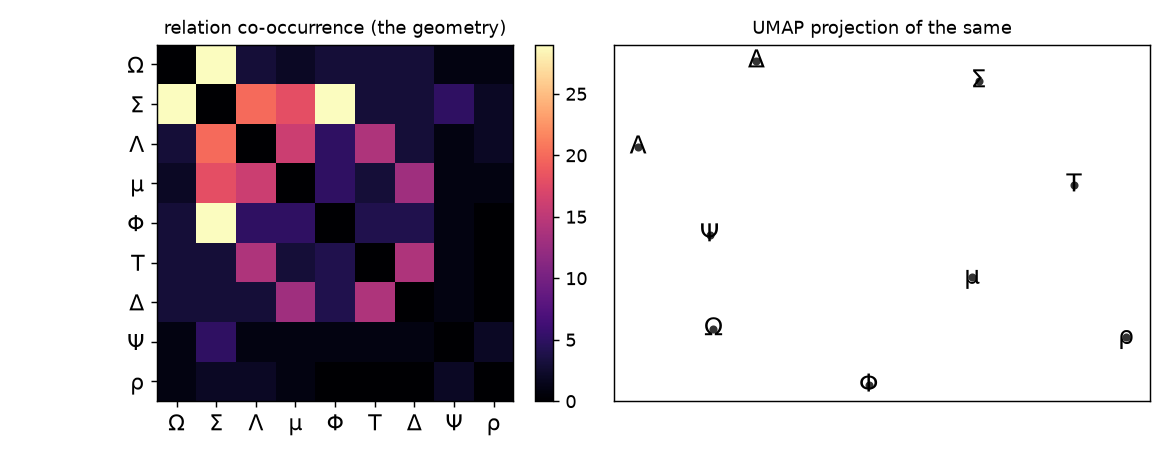
\includegraphics[width=0.92\textwidth]{manifold.png}
\caption{A projection of the relation co-occurrence across the lineage. Left: how often terms share a relation (\(\Sigma\) is densest). Right: a UMAP projection of the same geometry. This is a map of the authored structure --- where the terms sit relative to one another --- not a discovery of hidden meaning. Computed by an external prototype (\texttt{umap\_manifold.py}); the engine only embeds it.}\end{figure}
\section*{Symbolic weights (the trained network, written as glyphs)}
Each trained weight is stored as a fraction $h/c$ --- an Egyptian hieroglyph over a cuneiform sign --- normalized to the recorded range. The runtime reconstructs the network by decoding these glyphs; no binary blob is attached. It looks like esoteric mathematics; it is a quantized weight matrix, and the symbols are the numbers, not meaning.
\medskip\noindent $\Sigma$-module ($2{\to}2{\to}2$), 12 weights in range $[-2.45939,\,3.523463]$:
\[ \frac{\glyph{𓀍}}{\cunei{𒂟}}\;\frac{\glyph{𓅖}}{\cunei{𒅝}}\;\frac{\glyph{𓅓}}{\cunei{𒆔}}\;\frac{\glyph{𓄱}}{\cunei{𒇓}}\;\frac{\glyph{𓁁}}{\cunei{𒃤}}\;\frac{\glyph{𓀛}}{\cunei{𒄆}}\;\frac{\glyph{𓀁}}{\cunei{𒀏}}\;\frac{\glyph{𓂫}}{\cunei{𒂸}}\;\frac{\glyph{𓀁}}{\cunei{𒀁}}\;\frac{\glyph{𓃲}}{\cunei{𒅵}}\;\frac{\glyph{𓂍}}{\cunei{𒇄}}\;\frac{\glyph{𓀀}}{\cunei{𒀁}} \]
\section*{Evolution (this stage)}\noindent The oracle supplied the increment below; it was applied programmatically and recorded as data beside the questions --- not as answers to them.\par\medskip\noindent\textbf{Oracle (increment):}\VerbatimInput[fontsize=\small,frame=single]{_oracle_display.txt}\par\medskip\noindent\textbf{Application:} applied directly to self.dsl

\section*{Lineage and provenance}
This model extends its parent self-evolving inquiry, doi:local:self\_11, ingesting
its relations so the series can look fully back \cite{p6,paper1,paper2,p3}. The
companion papers set out the method and its discipline \cite{paper1,paper2,paper3}.
Actions record data beside questions; the document poses and enacts, and makes
no claim to resolve what a self is.
\section*{Appendix: self-extraction}
This PDF carries its engine (\texttt{introspecter8.py}), research module
(\texttt{research.py}), and DSL
(\texttt{self.dsl}) as embedded streams. Requires \texttt{pip install pypdf
numpy} and a LaTeX install. To produce the next stage, save and run:
\begin{Verbatim}[fontsize=\small,frame=single]
import base64
exec(base64.b64decode(
  "aW1wb3J0IHN5cywgZ2xvYiwgb3MKc3lzLnBhdGguaW5zZXJ0KDAsICIuIi"
  "kKZnJvbSBweXBkZiBpbXBvcnQgUGRmUmVhZGVyCmNhbmQgPSBOb25lCmZv"
  "ciBmIGluIGdsb2IuZ2xvYigiKi5wZGYiKToKICAgIHRyeTogYSA9IFBkZl"
  "JlYWRlcihmKS5hdHRhY2htZW50cwogICAgZXhjZXB0IEV4Y2VwdGlvbjog"
  "Y29udGludWUKICAgIGlmICJpbnRyb3NwZWN0ZXI4LnB5IiBpbiBhIGFuZC"
  "AoY2FuZCBpcyBOb25lIG9yIG9zLnBhdGguZ2V0bXRpbWUoZikgPiBvcy5w"
  "YXRoLmdldG10aW1lKGNhbmQpKToKICAgICAgICBjYW5kID0gZgpwZGYgPS"
  "BjYW5kIG9yIG1heChnbG9iLmdsb2IoIioucGRmIiksIGtleT1vcy5wYXRo"
  "LmdldG10aW1lKQpmb3IgbmFtZSwgZGF0YSBpbiBQZGZSZWFkZXIocGRmKS"
  "5hdHRhY2htZW50cy5pdGVtcygpOgogICAgb3BlbihuYW1lLCAid2IiKS53"
  "cml0ZShkYXRhWzBdIGlmIGlzaW5zdGFuY2UoZGF0YSwgbGlzdCkgZWxzZS"
  "BkYXRhKQppbXBvcnQgaW1wb3J0bGliLCBpbnRyb3NwZWN0ZXI4IGFzIEk7"
  "IGltcG9ydGxpYi5yZWxvYWQoSSk7IEkuZXZvbHZlKCkK"))
\end{Verbatim}
\begin{thebibliography}{9}
\bibitem{p6} B.~Hartshorn, \emph{Origin, Self, Language, Meaning, Other, Time,
and Difference: A Self-Evolving Hypergraph} (self\_6, parent).
doi:10.5281/zenodo.20710258
\bibitem{paper1} B.~Hartshorn, \emph{Staging the Question of Self: A
self-contained, self-modifying document that mixes poetry, philosophy, and
code}. doi:10.5281/zenodo.20709754
\bibitem{paper2} B.~Hartshorn, \emph{Enacting the Question of Self: Provenance,
a hypergraph, and a differentiable route that records computation as data}.
doi:10.5281/zenodo.20710444
\bibitem{p3} B.~Hartshorn, \emph{Origin, Self, Language, Meaning, Other, Time,
and Difference: A Self-Evolving Inquiry} (self\_3). doi:10.5281/zenodo.20707850
\bibitem{paper3} B.~Hartshorn, \emph{The Question of Self: Matrix Inscriptions
and Faux-Calculus}. doi:10.5281/zenodo.20814778
\bibitem{agi} B.~Hartshorn, \emph{Towards Self-Evolving AGI via Emergent DSL}.
viXra:2507.0104
\bibitem{meta} B.~Hartshorn, \emph{Emergent Self-Modification and
Meta-Programming in Dynamic Systems}. viXra:2507.0036
\bibitem{arch} B.~Hartshorn, \emph{Self-Contained Multi-AI Architecture
Definition via DSL}. viXra:2507.0074
\end{thebibliography}\end{document}
